\chapter{نتیجه گیری و پیشنهادات}
% \section{مقدمه}
% در این فصل، ما به بررسی نتایج بدست آمده و ارائه پیشنهاداتی می‌پردازیم که می‌توانند عملکرد سیستم کنترل پهپاد را از جنبه‌های مختلف بهبود بخشند. 
% نتایج به‌دست‌آمده در این پروژه نشان‌دهنده دقت بالای سیستم در تشخیص علائم‌ها و انتقال دستورات به پهپاد می‌باشد. با این حال، همچنان می‌توان بهبودهایی در عملکرد سیستم اعمال کرد تا دقت و کارایی آن افزایش یابد.
% این پیشنهادات شامل افزایش سرعت اجرای برنامه، بهبود دقت پیش‌بینی علائم‌ها و کاهش محدودیت‌های منابع 
% می‌باشند. هدف از این فصل، ارائه راهکارهای عملی و کاربردی است که بتوانند سیستم را به سطح بالاتری از کارایی و اطمینان برسانند.
\section{مقدمه}
در این فصل، ما به بررسی نتایج بدست آمده از این پروژه و ارائه پیشنهاداتی می‌پردازیم که می‌توانند عملکرد سیستم کنترل پهپاد را از جنبه‌های مختلف بهبود بخشند. نتایج به‌دست‌آمده در این پروژه نشان‌دهنده دقت بالای سیستم در تشخیص علائم‌ها و انتقال دستورات به پهپاد می‌باشد. با این حال، همچنان می‌توان بهبودهایی در عملکرد سیستم اعمال کرد تا دقت و کارایی آن افزایش یابد.
\\
این پیشنهادات شامل افزایش سرعت اجرای برنامه، بهبود دقت پیش‌بینی علائم‌ها و کاهش محدودیت‌های منابع می‌باشند. هدف از این فصل، ارائه راهکارهای عملی و کاربردی است که بتوانند سیستم را به سطح بالاتری از کارایی و اطمینان برسانند.


\section{نتیجه‌گیری}
نتایج به‌دست‌آمده در این پروژه نشان‌دهنده عملکرد دقیق و موفقیت‌آمیز آن است. این پروژه به تمامی اهداف از پیش تعیین‌شده، از جمله دقت بالا، صحت قابل قبول، فراخوانی مناسب، امتیاز \lr{F1} بالا، اجرای بی‌درنگ، رضایت کاربر، خطای پایین و قابلیت پیاده‌سازی بر روی پهپاد دست یافته است. عملکرد دقیق سیستم در تشخیص و کنترل پهپاد با استفاده از علائم‌های دست، نشان‌دهنده پتانسیل بالای این روش برای کاربردهای مختلف در صنعت و تکنولوژی است.


\section{پیشنهادات}
در این بخش پیشنهاداتی برای بهبود عملکرد پهپاد با کنترل دست بیان شده‌است.
\subsection{محدودیت وجود پهپاد‌های منبع‌باز}
در مورد محدودیت‌های استفاده از پهپادهای منبع‌باز و شرکتی برای پروژه کنترل پهپاد با استفاده از علائم دست بر مبنای بینایی ماشین، چندین موضوع موردنظر وجود دارد. 
\\
ابتدا، در مورد پهپادهای شرکتی، باید توجه داشت که این پهپادها معمولاً دارای سیستم‌های بسته و غیرقابل تغییر هستند که مانع از انجام تغییرات و سفارشی‌سازی‌های مورد نیاز برای اجرای الگوریتم‌های پیچیده بر روی آنها می‌شوند. همچنین، 
محدودیت‌های قانونی و مقرراتی مانند نیاز به مجوزهای خاص برای استفاده از پهپادهای تجاری در برخی کشورها می‌تواند چالش‌هایی را ایجاد کند.
\\
در مورد پهپادهای منبع‌باز، محدودیت‌های متفاوتی وجود دارد. این پهپادها ممکن است دارای سخت‌افزارهای قدرتمندی نباشند که بتوانند الگوریتم‌های پیچیده پردازش تصویر را اجرا کنند. همچنین، عدم پشتیبانی کامل از زبان‌های برنامه‌نویسی مدرن می‌تواند باعث پیچیدگی در توسعه و اجرای برنامه‌ها شود.
\\
با در نظر گرفتن این محدودیت‌ها، راهکار ساخت یک پهپاد سفارشی با سخت‌افزار مناسب و قابلیت برنامه‌نویسی مورد نیاز می‌تواند راه حلی مناسب باشد. این رویکرد امکان اجرای الگوریتم‌های پیچیده و پیاده‌سازی برنامه‌های سفارشی را فراهم می‌کند، که باعث بهبود کارایی و انعطاف‌پذیری سیستم در ارتباط با کنترل پهپاد با علائم دست خواهد شد.

\subsection{وجود چندین دست در تصویر}
وجود چندین دست در تصویر یک چالش بزرگ در برنامه است. در این مورد باید به این نکته توجه کنیم که در یک فریم تصویر، ممکن است چندین دست قابل مشاهده باشند که این می‌تواند برای الگوریتم‌های تشخیص دست مشکل‌ساز شود. زیرا 
الگوریتم‌ها باید بتوانند دست‌ها را تفکیک کرده و علائم‌های متفاوت آنها را تشخیص دهند. همچنین ممکن است دست‌های غیرمرتبط با کاربر، مانند دست‌های در پس‌زمینه یا دست‌های دیگر افراد، نیز در تصویر حضور داشته باشند که این موضوع می‌تواند دقت الگوریتم را کاهش دهد.
\\
یکی از راهکارهای موردنظر برای حل این چالش، شخصی‌سازی مدل تشخیص دست با توجه به داده‌هایی که از کاربران جمع‌آوری می‌شود، است. این روش می‌تواند به کمک داده‌های جمع‌آوری شده از دست‌های واقعی کاربران، به مدل کمک 
کند تا الگوهای مختلف دست‌ها را بیشتر بشناسد و از این طریق دقت تشخیص را افزایش دهد. با این حال، این روش نیازمند زمان و تلاش برای جمع‌آوری و برچسب‌گذاری داده‌های موردنیاز است و ممکن است برای کاربران خوشایند نباشد.
\\
راهکار دیگری که می‌توان برای حل این مسئله در نظر گرفت، استفاده از یک سیستم ارتباطی میان دست و پهپاد است. به این ترتیب، کاربر می‌تواند یک دستبند یا سیمی را در دست خود داشته باشد که این دستبند به عنوان نشانه تشخیص دست و 
ارتباط بین کاربر و پهپاد عمل کند. با این روش، پهپاد تنها دستی را که دارای دستبند است شناسایی می‌کند و به دستورات آن پاسخ می‌دهد. این راهکار می‌تواند از دقت و سرعت الگوریتم تشخیص بهره‌مند شود و به کاربر اطمینان بیشتری بدهد. با 
این حال، برای اجرای این روش نیازمند توسعه و اعمال یک مدل دیگر برای تشخیص دست با دستبند است که این می‌تواند زمان و هزینه بیشتری را به بار آورد.


\subsection{شناسایی یک دست در دو مستطیل در نتیجه دو خروجی دست}
یکی از مشکلاتی که بسیاری از استفاده‌کنندگان کتابخانه مدیاپایپ با آن مواجه شده‌اند، مربوط به شناسایی یک دست با دو مستطیل متفاوت و در نتیجه دو خروجی است. این مشکل می‌تواند به علت همپوشانی بین دو مستطیلی که دست را 
شناسایی می‌کنند، ایجاد شود. با این حال، این مشکل برای پروژه خاصی که ما در دست داریم تفاوتی ایجاد نکرده است، زیرا ما یک گزینه را انتخاب کرده و علائم دست را در آن پیش‌بینی می‌کنیم.
\\
اما از بین بردن این مشکل می‌تواند با بهبود و بهینه‌سازی کارایی این کتابخانه را برای سایر استفاده‌کنندگان افزایش دهد. برای حل این مشکل، می‌توان محدودیتی برای همپوشانی مستطیل‌های حاوی دست را در نظر گرفت. به این صورت که اگر دو مستطیل بیشتر از حد در نظر گرفته شده 
همپوشانی داشته باشند، یعنی یک دست در دو تصویر تشخیص داده شده باشد، تنها یکی از آنها به مدل بعدی ارسال شود. این روش می‌تواند به استفاده‌کنندگان دیگر از کتابخانه مدیاپایپ کمک کند تا با مشکلاتی از این دست مواجه نشوند و از امکانات بهتری برای تشخیص دست بهره‌مند شوند.

\begin{figure}[h]
    \centering
    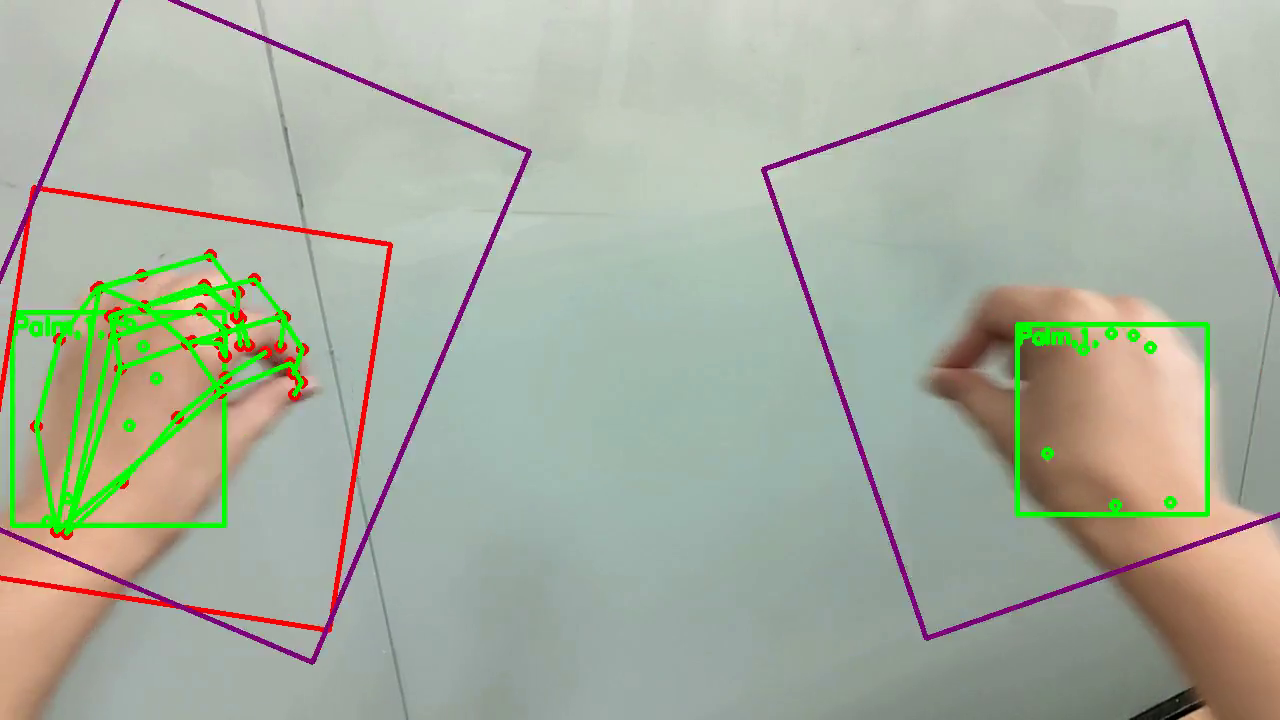
\includegraphics[width=0.6\textwidth]{multi_boxes.png}
    \caption{شناسایی یک دست دو مرتبه}
\end{figure}


\subsection{اجرا بر روی پردازنده‌های گرافیکی }
پروژه ما  به علت عدم در دسترس بودن پهپادی که از پردازنده‌های گرافیکی برای اجرای مدل‌ها استفاده کند, به صورتی پیاده‌سازی شده است که تنها بر روی پردازنده مرکزی قابل اجرا است. با این حال، اگر پهپادی با توانایی اجرای مدل‌ها بر روی 
پردازنده‌های گرافیکی در دسترس باشد، سه مدل که به صورت پی‌در‌پی اجرا می‌شوند می‌توانند بر روی پردازنده‌های گرافیکی اجرا شده تا عملکرد سیستم را بهبود بخشیده و تجربه کاربری را بهبود بخشند. استفاده از پردازنده‌های گرافیکی برای اجرای مدل‌ها می‌تواند 
سرعت پردازش را بسیار افزایش دهد، زیرا کارت‌های گرافیکی معمولاً دارای تعداد زیادی هسته محاسباتی هستند که برای پردازش موازی و سریع داده‌ها بسیار مناسب هستند. این امر می‌تواند منجر به بهبود قابل توجهی در زمان پاسخ و دقت 
تشخیص علائم دست شود و تجربه کاربری را بهبود بخشد. به علاوه، با استفاده از پردازنده‌های گرافیکی، می‌توانیم بار محاسباتی را از پردازنده مرکزی کاهش داده و عملکرد کلی سیستم را بهبود بخشیم.

\subsection{اجرای پروژه با برنامه سی پلاس پلاس}
با توجه به مزایای زبان سی پلاس پلاس نسبت به پایتون، انتخاب این زبان برای انجام این پروژه می‌تواند به بهبود عملکرد و کارایی سیستم کمک شایانی کند. در ادامه به برخی از مزایای استفاده از زبان سی پلاس پلاس نسبت به پایتون در این پروژه پرداخته شده است:

\begin{itemize}
    \item عملکرد و سرعت اجرای بالا: سی پلاس پلاس یک زبان برنامه‌نویسی کامپایل‌شده است که به کد ماشین تبدیل می‌شود، به همین دلیل عملکرد و سرعت اجرای بسیار بالاتری نسبت به پایتون دارد که یک زبان تفسیری است. این ویژگی
    برای پروژه‌های بی‌درنگ مانند کنترل پهپاد با استفاده از علائم دست بسیار حیاتی است، زیرا زمان پاسخ‌دهی سریع و دقیق در این سیستم‌ها اهمیت زیادی دارد.
    \item مدیریت دقیق حافظه: سی پلاس پلاس امکان مدیریت دقیق حافظه را فراهم می‌کند. این ویژگی می‌تواند بهینه‌سازی استفاده از منابع سیستم و کاهش مصرف حافظه را به دنبال داشته باشد، که برای سیستم‌هایی 
    با منابع محدود مانند پهپادها بسیار مهم است. مدیریت صحیح حافظه می‌تواند به جلوگیری از نشت حافظه و افزایش پایداری سیستم کمک کند.
    \item کتابخانه‌ها و چارچوب‌های قدرتمند: سی پلاس پلاس دارای کتابخانه‌ها و چارچوب‌های قدرتمندی برای پردازش تصویر و بینایی ماشین مانند اپن سی‌وی است. اپن سی‌وی به زبان سی پلاس پلاس نوشته شده
    و عملکرد بهتری نسبت به معادل‌های پایتونی خود دارد. این کتابخانه قابلیت‌های متعددی را برای پردازش تصاویر، شناسایی و تشخیص اشیا فراهم می‌کند که می‌تواند در پروژه‌های بینایی ماشین بسیار موثر باشد.
    \item دسترسی و کنترل سطح پایین سخت‌افزار: سی پلاس پلاس امکان دسترسی و کنترل سطح پایین سخت‌افزار را فراهم می‌کند. این ویژگی برای کنترل مستقیم پهپاد و بهینه‌سازی ارتباط با سنسورها 
    و موتورها بسیار مفید است. با استفاده از سی پلاس پلاس می‌توان به طور مستقیم با اجزای سخت‌افزاری پهپاد ارتباط برقرار کرده و عملکرد سیستم را بهینه کرد.
    \item  پشتیبانی قوی از چندریسمانی \LTRfootnote{Multithreading}: سی پلاس پلاس پشتیبانی قوی‌تری از چندریسمانی و پردازش موازی دارد. این قابلیت می‌تواند برای بهبود کارایی و پاسخ‌دهی سریع در پردازش‌های پیچیده بینایی ماشین 
    و کنترل پهپاد بسیار مهم باشد. با استفاده از چندریسمانی، می‌توان عملیات مختلف را به صورت همزمان انجام داد و زمان اجرای کل سیستم را کاهش داد.
\end{itemize}

\subsection{استفاده از مدل‌های موازی برای تشخیص علائم دست}
برای بهبود دقت و کارایی پروژه کنترل پهپاد با استفاده از علائم دست، می‌توان از رویکردی مبتنی بر اجرای موازی مدل‌ها بهره برد. در این روش، تصویر تشخیص داده شده از دست به طور همزمان به دو مدل با معماری‌های مختلف ارسال 
می‌شود. به عنوان مثال، یک مدل می‌تواند از معماری شبکه‌های عصبی پیچشی و مدل دیگر از معماری حافظه بلندمدت کوتاه‌مدت استفاده کند. تنها در صورتی که هر دو مدل تشخیص یکسانی از علائم دست داشته باشند، 
دستور نهایی به پهپاد ارسال می‌شود. این رویکرد می‌تواند به طور قابل توجهی دقت تشخیص علائم دست را افزایش دهد و ریسک‌های مالی مرتبط با اشتباهات تشخیصی را کاهش دهد.

\subsection{توسعه برنامه با استفاده از سایر قسمت‌های بدن انسان}
یکی از مسیرهای جذاب برای توسعه آینده پروژه کنترل پهپاد با علائم دست، گسترش سیستم به گونه‌ای است که بتوان از قسمت‌های دیگر بدن انسان برای کنترل حرکت پهپاد استفاده کرد. این رویکرد می‌تواند به ایجاد تعاملات طبیعی‌تر و راحت‌تر بین کاربر و پهپاد منجر شود. در زیر به برخی از این ایده‌ها و مزایای آن‌ها پرداخته می‌شود.
\\
\subsubsection{کنترل پهپاد با حرکات چشم}
یکی از نوآورانه‌ترین روش‌ها برای کنترل پهپاد، استفاده از حرکات چشم کاربر است. این سیستم می‌تواند به وسیله ردیابی حرکت چشم کاربر، مکانی نسبی را که کاربر به آن نگاه می‌کند، شناسایی کرده و پهپاد را به سمت آن نقطه هدایت کند. برای پیاده‌سازی این روش، از تکنیک‌های پیشرفته بینایی ماشین و ردیابی چشم استفاده می‌شود.
\\
استفاده از حرکات چشم برای کنترل پهپاد مزایای متعددی دارد. این روش می‌تواند دقت و کارایی سیستم را افزایش دهد، زیرا حرکات چشم نقاط دقیق‌تری را نسبت به حرکات دست مشخص می‌کنند. این امر به پهپاد امکان می‌دهد تا با دقت بیشتری به نقاط مورد نظر حرکت کند. علاوه بر این، استفاده از چشم برای 
کنترل پهپاد می‌تواند بسیار طبیعی‌تر و راحت‌تر از حرکات دست باشد، به ویژه در شرایطی که دست‌ها مشغول هستند یا امکان استفاده از آن‌ها وجود ندارد. این روش همچنین می‌تواند خستگی ناشی از استفاده مداوم از دست‌ها برای کنترل پهپاد را کاهش دهد، که در نتیجه تجربه کاربری بهتری را فراهم می‌کند.

\subsubsection{کنترل پهپاد با حرکات سر}
روش دیگر برای کنترل پهپاد، استفاده از حرکات سر است. در این سیستم، کاربر می‌تواند با چرخش سر به جهات مختلف، مسیر حرکت پهپاد را تعیین کند. حرکات سر به طور طبیعی و بدون نیاز به تجهیزات اضافی قابل انجام هستند، که این امر تعامل با پهپاد را
ساده‌تر می‌کند. استفاده از حرکات سر به ویژه در محیط‌هایی که استفاده از دست‌ها ممکن نیست (مثل محیط‌های کاری خاص یا شرایط پزشکی) بسیار مفید است. این روش می‌تواند به سادگی و طبیعی بودن تعامل با پهپاد کمک کند و تجربه کاربری را بهبود بخشد.

\section{جمع‌بندی}
در این فصل، به نتیجه‌ بدست آمده و بررسی چندین چالش‌ و محدودیت‌های سیستم کنترل پهپاد پرداخته‌شد و راهکارهای متعددی برای بهبود عملکرد آن ارائه شد. 
\\
اولین محدودیت، استفاده از پهپادهای منبع‌باز است که با وجود مزایای فراوان، ممکن است دارای محدودیت‌های سخت‌افزاری و نرم‌افزاری باشند. برای غلبه بر این محدودیت، پیشنهاد شد که از پهپادهای با قابلیت‌های پیشرفته‌تر و 
بهینه‌سازی کدهای نرم‌افزاری استفاده شود. همچنین، راهکارهایی برای مدیریت چندین دست در تصویر و جلوگیری از شناسايي نادرست یک دست در دو مستطیل ارائه شد که می‌تواند دقت سیستم را بهبود بخشد.
\\
در ادامه، به اهمیت اجرای پروژه روی پردازنده‌های گرافیکی و برنامه‌نویسی به زبان سی پلاس پلاس پرداختیم که می‌تواند سرعت اجرای برنامه را افزایش دهد. استفاده از مدل‌های موازی برای تشخیص علائم دست نیز به‌عنوان یک راهکار مؤثر برای بهبود 
دقت و سرعت پیشنهاد شد. همچنین، روش‌های جدیدی مانند کنترل پهپاد با حرکات چشم و سر معرفی شدند که امکانات بیشتری برای کاربران فراهم می‌کنند.
\\
در نتیجه، با توجه به بررسی‌ها و پیشنهادات ارائه شده در این فصل، می‌توان انتظار داشت که با اعمال این بهبودها، سیستم کنترل پهپاد به سطح بالاتری از کارایی و اطمینان دست یابد. این راهکارها نه‌تنها عملکرد سیستم را بهبود می‌بخشند، بلکه تجربه کاربری بهتری را نیز فراهم می‌آورند.